\begin{comment}
\end{comment}

\chapter{Simulation de circuits quantiques avec les réseaux de tenseurs}
\label{ann:simulation-circuits-quantiques-avec-reseaux-de-tenseurs}

La simulation classique d'états quantiques est tout sauf évidente. Ces états, appartenant à l'espace de Hilbert, sont décrit par des vecteurs d'état de taille exponentielle empêchant ainsi leur caractérisation même pour des systèmes de taille modeste. Cette difficulté, présente dans de nombreux domaines telle l'apprentissage-machine, est aussi connue sous le nom de la \textit{malédiction de la dimensionnalité}. Cependant, la représentation de certains états physiques intéressants contient parfois de l'information superflue ou une structure inhérente. Par exemple, un état quantique général de $n$ qubits requiert en théorie un vecteur d'état à $2^{n}$ bits, mais un état quantique non intriqué nécessite seulement $2n$ bits en raison de l'absence de corrélation. Cette idée a alors mené au développement des méthodes de réseaux de tenseurs pour l'étude de système quantique à plusieurs corps en matière condensé afin d'obtenir une représentation des états quantiques plus efficace. 

Cette annexe décrit seulement en surface les méthodes de réseaux de tenseur. Pour comprendre les différentes méthodes plus en profondeur, de nombreux excellents tutoriels ont été écrits~\cite{bridgemanHandwavingInterpretiveDance2017,biamonteTensorNetworksNutshell2017,bakerMethodesCalculAvec2021}. La section~\ref{sec:reseaux-de-tenseurs} introduit les réseaux de tenseurs ainsi que les principales opérations possibles. Une représentation alternative de ceux-ci, les états en produits de matrice, sont décrit à la section~\ref{sec:mps-mpo} alors que la correspondance entre la simulation de circuits quantiques et la contraction de réseaux de tenseurs est expliqué à la section~\ref{sec:simulation-de-circuits-quantiques}.

%-----------------------------------------------------------------------------%

\section{Réseaux de tenseurs}
\label{sec:reseaux-de-tenseurs}

Un \textit{tenseur} est un tableau multilinéaire avec un rang, c'est-à-dire un nombre de dimensions, arbitraire encodant une certaine quantité d'information. Par exemple, un scalaire, un vecteur et une matrice correspondent respectivement à un tenseur de rang 0, 1 et 2. Les tenseurs généralisent en outre ces derniers objets en admettant des tenseurs de rang $m$. Plus formellement, un tenseur $T[x_{1}, x_{2}, \dots, x_{m}]$ de rang $m$ avec dimensions $d_{1} \times d_{2} \times \dots \times d_{m}$ est un élément de l'ensemble $\mathbb{C}^{d_{1} \times d_{2} \times \dots \times d_{m}}$. Les tenseurs s'interprètent aussi comme une fonction définie sur un domaine discret. L'utilité principale des tenseurs est leur représentation géométrique simple, qui permet de visualiser aisément leurs caractéristiques principales et de faciliter leur manipulation. Tout tenseur se représente par une forme géométrique, où chaque indice $x_{i}$ est illustré avec une patte sortant de la forme tel qu'illustré à la figure~\ref{fig:tensor}

\begin{figure}[ht!]
    \centering
    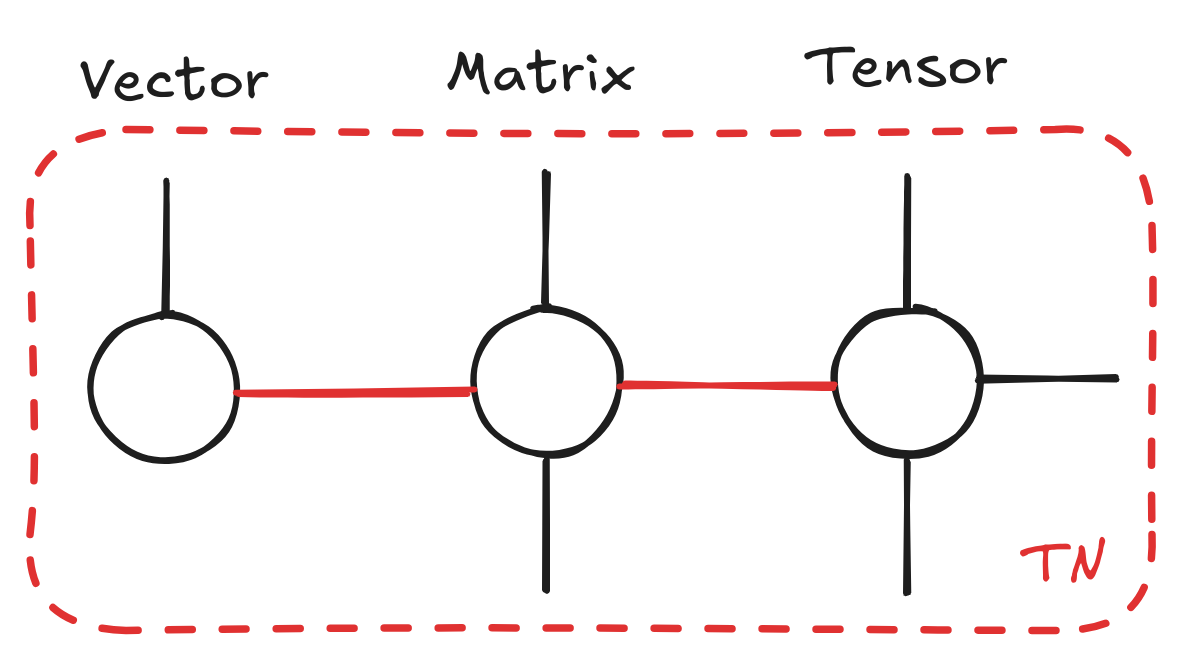
\includegraphics[width=0.6\textwidth]{figures/tensor.png}
    \caption{}
    \label{fig:tensor}
\end{figure}

Plusieurs opérations peuvent être appliquées sur des tenseurs. Le produit tensoriel juxtapose 


La contraction de deux tenseurs 

D'autres opérations sont aussi importantes. La trace d'un tenseur est la sommation sur les

D'autres opérations, comme la trace, la décomposition, le regroupement et la séparation.

Un réseau de tenseurs est une collection de tenseurs $\set{ T_{1}[\varepsilon_{1}], T_{2}[\varepsilon_{2}], \dots, T_{n}[\varepsilon_{n}] }$ pour $\varepsilon_{i} \subset \set{ x_{1}, x_{2}, \dots, x_{m} }$ partageant certains indices $x_{i}$. La notation en réseaux de tenseurs s'apparente beaucoup à la notation d'Einstein. 




%-----------------------------------------------------------------------------%

\section{État en produit de matrices et opérateur en produit de matrices}
\label{sec:mps-mpo}

Un \textit{état en produit de matrices} (« Matrix Product State ») (MPS) est une représentation efficace d'un état quantique.




%-----------------------------------------------------------------------------%

\section{Simulation de circuits quantiques}
\label{sec:simulation-de-circuits-quantiques}

\begin{comment}
\subsection*{Plan}

\begin{enumerate}
    \item Décrire le lien entre les circuits quantiques et les réseaux de tenseurs
    \item Décrire les différentes méthodes de simulation (MPS-MPO et réseau de tenseurs général)
    \item Décrire la méthode d'échantillonage
\end{enumerate}

\subsection*{Références}

1. Gray, J. quimb: A python package for quantum information and many-body calculations. Journal of Open Source Software 3, 819 (2018).

2. Ferris, A. J. and Vidal, G. Perfect Sampling with Unitary Tensor Networks. Phys. Rev. B 85, 165146 (2012).
\end{comment}


Afin d'obtenir des échantillons à partir d'un réseau de tenseur, deux méthodes sont possibles. D'abord, une réprésentation dense de la fonction d'onde peut être obtenue en contractant le réseau. Les états sont alors simplement obtenus en pigeant selon la distribution de probabilité trouvée. Une méthode alternative utilise plutôt ~\cite{ferrisPerfectSamplingUnitary2012}. 






%-----------------------------------------------------------------------------%
